% `template.tex', a bare-bones example employing the AIAA class.
%
% For a more advanced example that makes use of several third-party
% LaTeX packages, see `advanced_example.tex', but please read the
% Known Problems section of the users manual first.
%
% Typical processing for PostScript (PS) output:
%
%  latex template
%  latex template   (repeat as needed to resolve references)
%
%  xdvi template    (onscreen draft display)
%  dvips template   (postscript)
%  gv template.ps   (onscreen display)
%  lpr template.ps  (hardcopy)
%
% With the above, only Encapsulated PostScript (EPS) images can be used.
%
% Typical processing for Portable Document Format (PDF) output:
%
%  pdflatex template
%  pdflatex template      (repeat as needed to resolve references)
%
%  acroread template.pdf  (onscreen display)
%
% If you have EPS figures, you will need to use the epstopdf script
% to convert them to PDF because PDF is a limmited subset of EPS.
% pdflatex accepts a variety of other image formats such as JPG, TIF,
% PNG, and so forth -- check the documentation for your version.
%
% If you do *not* specify suffixes when using the graphicx package's
% \includegraphics command, latex and pdflatex will automatically select
% the appropriate figure format from those available.  This allows you
% to produce PS and PDF output from the same LaTeX source file.
%
% To generate a large format (e.g., 11"x17") PostScript copy for editing
% purposes, use
%
%  dvips -x 1467 -O -0.65in,0.85in -t tabloid template
%
% For further details and support, read the Users Manual, aiaa.pdf.


% Try to reduce the number of latex support calls from people who
% don't read the included documentation.
%

% FVPR = FLIR Vue Pro R. Not sure if we want to reference as FLIR after the first inclusion



\typeout{}\typeout{If latex fails to find aiaa-tc, read the README file!}
%

\documentclass[]{aiaa-tc}% insert '[draft]' option to show overfull boxes

\usepackage{pdfpages}
\usepackage{url}
\usepackage{color}			% \textcolor
\usepackage{multirow}
\usepackage{subfigure}  % subcaptions for subfigures
\usepackage{subfigmat}  % matrices of similar subfigures, aka small mulitples
\usepackage{float}      % allows pictures to float
\usepackage{graphicx} 
\usepackage{array,booktabs,calc}
\newcolumntype{L}[1]{>{\raggedright\let\newline\\\arraybackslash\hspace{0pt}}m{#1}}
\newcolumntype{C}[1]{>{\centering\let\newline\\\arraybackslash\hspace{0pt}}m{#1}}
\newcolumntype{R}[1]{>{\raggedleft\let\newline\\\arraybackslash\hspace{0pt}}m{#1}}
\renewcommand{\figurename}{Fig.} %changes Figure. to Fig.

 \title{Trailing External Measurements for Pressure Measurements: Improved Trailing Pressure Measurement System for Onboard Sensor Calibration }
\author{
%
Zachary Rotter
  \thanks{Undergraduate, Department of Aeronautics and Astronautics, Seattle, WA 98195, AIAA Student Member.},
  Kirby Taylor%
    \thanksibid{1},
    Laura Smit%
    \thanksibid{1},
  Bohao Zhu,%
  \thanksibid{1},
  \\
  {\normalsize\itshape
   Autonomous Flight Systems Laboratory, University of Washington, Seattle, WA, 98195, USA}\\
  \and
  Todd Leighton,%
   \thanks{Flight Test and Design Engineer, AeroTEC - Aerospace Testing Engineering and Certification L.L.C, Inc., Seattle, WA, 98108}\\
  {\normalsize\itshape
  AeroTEC L.L.C., Seattle, WA, 98108, USA}\\
  \and
  Christopher W. Lum%
   \thanks{Research Assistant Professor, Department of Aeronautics and Astronautics, Seattle, WA 98195, Member AIAA.}\\
  {\normalsize\itshape
  Autonomous Flight Systems Laboratory, University of Washington, Seattle, WA, 98195, USA}
 }

 % Data used by 'handcarry' option if invoked
 \AIAApapernumber{YEAR-NUMBER}
 \AIAAconference{Conference Name, Date, and Location}
 \AIAAcopyright{\AIAAcopyrightD{YEAR}}

 % Define commands to assure consistent treatment throughout document
 \newcommand{\eqnref}[1]{(\ref{#1})}
 \newcommand{\class}[1]{\texttt{#1}}
 \newcommand{\package}[1]{\texttt{#1}}
 \newcommand{\file}[1]{\texttt{#1}}
 \newcommand{\BibTeX}{\textsc{Bib}\TeX}

\begin{document}

\maketitle

\begin{abstract}
	This paper describes the design, manufacturing, testing, and evaluation of an automated trailing pressure measurement system for Part 23 and Part 25 aircraft flight testing. The primary goal of the system  is to measure static and total pressure of the atmospheric conditions of aircraft being subjected to Reduced Vertical Separation Minimum (RVSM) certification. The system utilizes a series of pitot tubes that relay information to a Paroscientific Series 2000 Absolute Pressure Transducer and a Honeywell Precision Differential Pressure Transducer. In addition to detailing the engineering design of the drogue, this paper outlines the testing campaign to validate its functionality.
\end{abstract}

\section*{Nomenclature}\label{sec:nomenclature}
\textcolor{red}{CL - Need to update with 'fuselage', 'board', 'primary aircraft', etc. (these are just placeholder names, what goes in the table below should be agreed upon and finalized with the team}.
\begin{tabbing}
  XXXXXXXXXX \= \kill% this line sets tab stop
  $A$		\> Surface area in $\textrm{m}^2$ \\
  AFSL 		\> Autonomous Flight Systems Laboratory \\
  $C_{D}$	\> Drag coefficient \\
  $D$		\> Drag force in lbs \\
  DGPS 		\> Differential Global Positioning System \\
  Drogue	\> Physical trailing pressure measurement system \\
  Fins		\> Plastic symmetrical airfoils on the rear end of the fuselage \\
  Fuselage		\> Aluminum tube that comprises the midsection of the drogue \\
  Housing		\> Aluminum tube attached to the primary aircraft that houses the drogue when it is not trailing \\
  Nose cone		\> Plastic cone attached to the front of the fuselage \\
  Payload		\> All electronic components on the plywood board inside the drogue \\
  Payload mount		\> Metal angles that keep the payload in place \\
  Primary aircraft		\> Aircraft the drogue trails behind \\
  $\rho$	\> Density in $\textrm{kg/m}^3$ \\
  Tail cone		\> Plastic cone attached to the rear of the fuselage \\
  UW 		\> University of Washington \\
  $v$	\> Velocity in m/s \\
  Winch		\> Motor and reel that lets out the drogue and returns it to the housing\\
%   [5pt]
%   \textit{Subscript}\\
%   $i$ \> Variable number \\
 \end{tabbing}


\section{Introduction}
\label{sec:introduction}

%%%%%%%%%%%%%%%%%%%%%%%%%%%%%%%%%%%%%%%%%%%%%%%%%%%%%%%%%%%%%%%%%%%%%%%%%%%%%%%%%%%%
\subsection{Problem Statement}
\textcolor{red}{LS to talk about about what we are trying to do and why this is difficult}

% What is the drogue
The purpose of this project was to design a pressure measurement system external to the aircraft. This system will be referred to as the drogue. The drogue was designed to be towed behind an aircraft in the free-stream air. The pressure measurements taken by the drogue were intended to be the true static and total pressure at a given altitude, as opposed to the measurements taken by the aircraft which are influenced by the aircraft itself. These true pressure measurements would then be used to calibrate the aircraft's pressure measurement instruments during flight tests of the aircraft.\\  

This drogue was intended to be an upgrade of the current static pressure measurement systems used during flight testing. The requirements for the drogue as laid out at the onset of this project focused on maintaining the accuracy and flight test length while reducing the modifications necessary to use the new system. Specifically, the drogue was required to measure the static pressure within 90\% accuracy of the current system in addition to tying with the data acquisition systems used currently and having power for up to four hours of flight time. In addition, the new design must be usable on Part 23-25 aircraft, be usable at all of the speeds these aircraft are tested, and require fewer modifications to install than the current systems.\\

From these requirements, additional specifications were drawn. In order to reduce the attachment modifications, the drogue must be a self-contained system. All pressure transducers and power systems must be within the drogue itself. In addition, the winch system which would reel the drogue in and out must be located in the drogue. In order to retain the current accuracy of pressure measurements, the body of the drogue must have a low pressure influence where ever the pressure was measured from. The drogue must also make minimal movements while in flight which would reduce the accuracy of the pressure measurements. This could be fulfilled either by natural stability or an active control system. A wireless transmission system must be used for real time transferal of the pressure measurements and the drogue must have a way of locating its position relative to the aircraft.\\ 

     
%%%%%%%%%%%%%%%%%%%%%%%%%%%%%%%%%%%%%%%%%%%%%%%%%%%%%%%%%%%%%%%%%%%%%%%%%%%%%%%%%%%%

%%%%%%%%%%%%%%%%%%%%%%%%%%%%%%%%%%%%%%%%%%%%%%%%%%%%%%%%%%%%%%%%%%%%%%%%%%%%%%%%%%%%
\subsection{Literature Review}
\textcolor{red}{ZR and KT - Talk about what other people have done in this space.  Cite papers like this\cite{Lum_Risk_for_UAVs_2010}}

% System currently in use?
	% Trailing Cones
	% Flying bomb
%%%%%%%%%%%%%%%%%%%%%%%%%%%%%%%%%%%%%%%%%%%%%%%%%%%%%%%%%%%%%%%%%%%%%%%%%%%%%%%%%%%%

\section{Experimental Methods}
\label{sec:ExperimentalMethods}

%%%%%%%%%%%%%%%%%%%%%%%%%%%%%%%%%%%%%%%%%%%%%%%%%%%%%%%%%%%%%%%%%%%%%%%%%%%%%%%%%%%%
\subsection{Ground Testing}
\textcolor{red}{CL  - Discuss how we will do ground testing.  Do not put results of these tests here as we have a separate section for results.}

%%%%%%%%%%%%%%%%%%%%%%%%%%%%%%%%%%%%%%%%%%%%%%%%%%%%%%%%%%%%%%%%%%%%%%%%%%%%%%%%%%%%

%%%%%%%%%%%%%%%%%%%%%%%%%%%%%%%%%%%%%%%%%%%%%%%%%%%%%%%%%%%%%%%%%%%%%%%%%%%%%%%%%%%%
\subsection{Flight Testing}
\textcolor{red}{CL  - Discuss how we will do flight testing.  Do not put results of these tests here as we have a separate section for results.}

%%%%%%%%%%%%%%%%%%%%%%%%%%%%%%%%%%%%%%%%%%%%%%%%%%%%%%%%%%%%%%%%%%%%%%%%%%%%%%%%%%%%


\section{Results}
\label{sec:Results}

%%%%%%%%%%%%%%%%%%%%%%%%%%%%%%%%%%%%%%%%%%%%%%%%%%%%%%%%%%%%%%%%%%%%%%%%%%%%%%%%%%%%
\subsection{Ground Testing}
\textcolor{red}{CL  - Discuss results from ground testing.}
During each run of the ground test, a Pixhawk data acquisition system was used to collect data on the motion of the drogue while in flight. This data was then converted to Euler angles and axial accelerations for additional analysis. Fig. \ref{fig:Run2Euler} shows the Euler angles from the drogue in Configuration 1, while Fig. \ref{fig:Run4Euler} shows the drogue in Configuration 2 and Fig. \ref{fig:Run6Euler} shows the drogue in Configuration 3. Though this figure shows all three Euler angles, analysis was focused on the Roll angle, which is the top plot in all three figures.

\begin{figure}
	\centering
	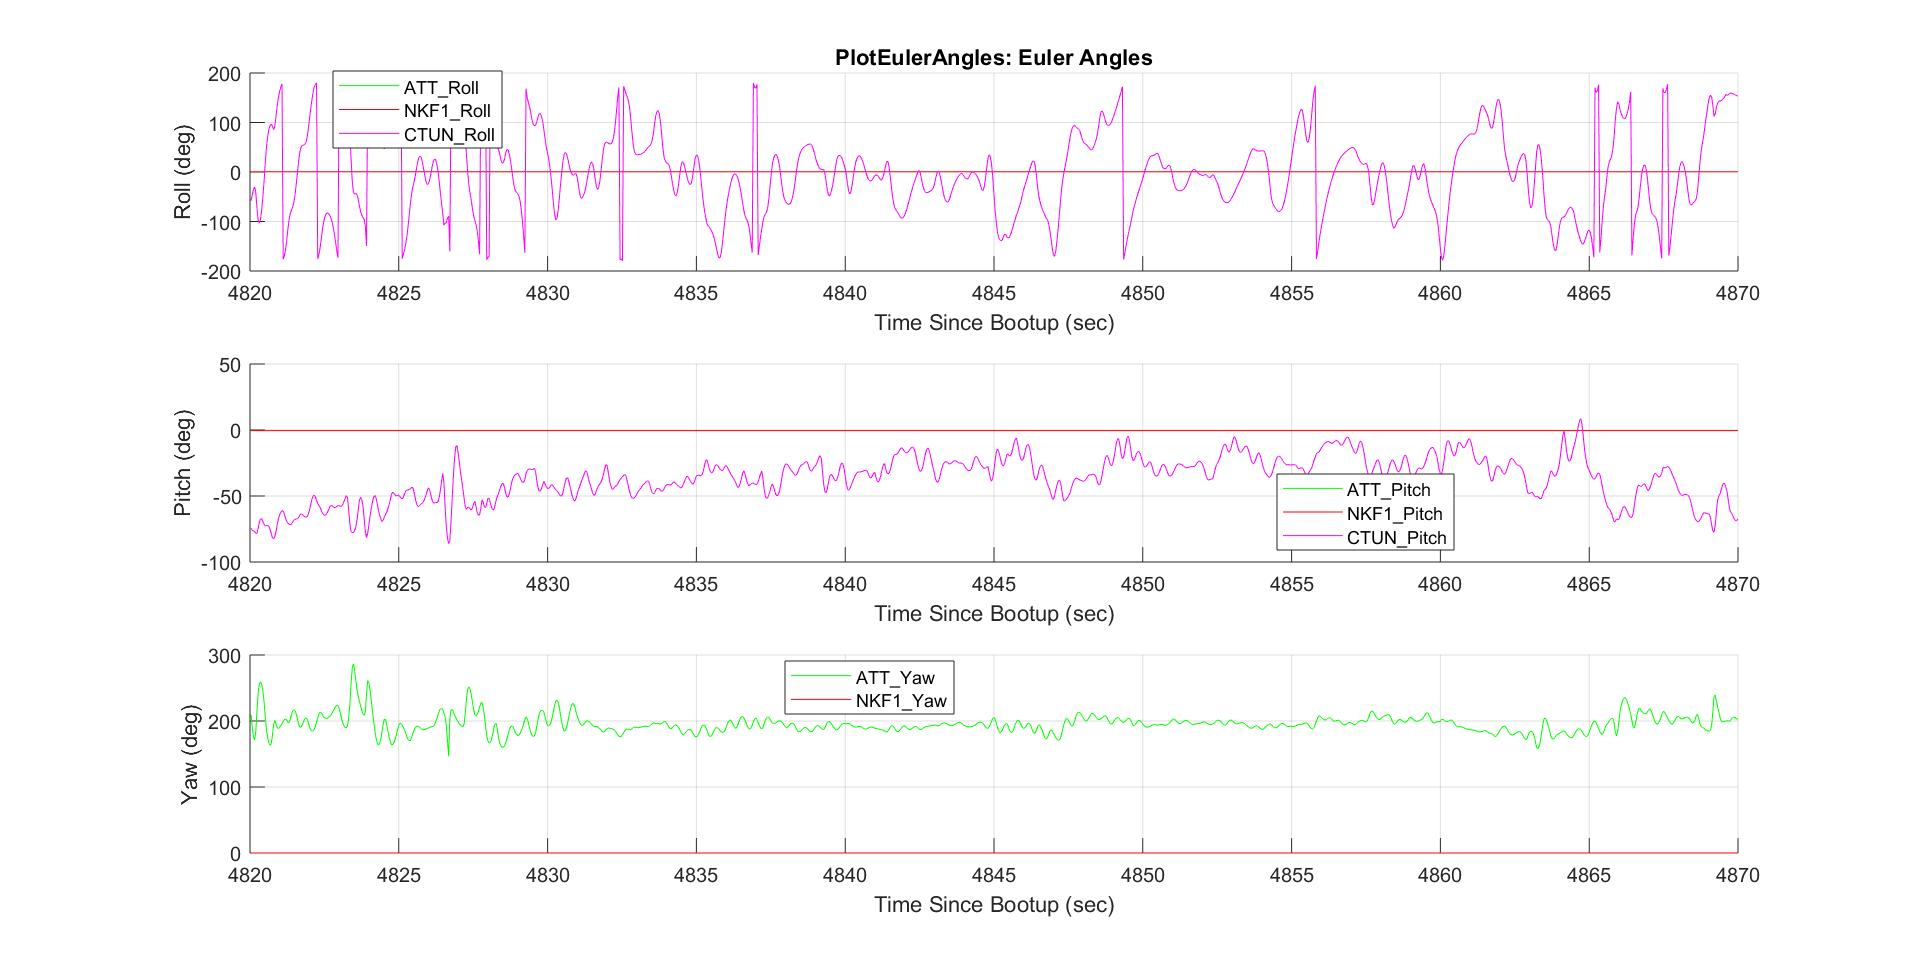
\includegraphics[width=1\linewidth]{./images/Run2_Euler}
	\caption{Euler angles in Configuration 1.} %way to classify fins
	\label{fig:Run2Euler}
\end{figure}

Each test includes a very short window of time when the drogue was moving through the air at a high enough speed to simulate actual flight tests. For Fig. \ref{fig:Run2Euler}, was identified as occurring approximately between times 4830 $sec$ and 4865 $sec$. Because the truck reached lower speeds during this test than the other tests, the flight time for this run was significantly shorter than the other tests. When looking at the Euler angles in this time frame, complete rolls by the drogue are shown by vertical lines stretching from 200 $deg$ to -200 $deg$. During this time frame 4 rolls were identified. 

%%%%%%%%%%%%%%%%%%%%%%%%%%%%%%%%%%%%%%%%%%%%%%%%%%%%%%%%%%%%%%%%%%%%%%%%%%%%%%%%%%%%

%%%%%%%%%%%%%%%%%%%%%%%%%%%%%%%%%%%%%%%%%%%%%%%%%%%%%%%%%%%%%%%%%%%%%%%%%%%%%%%%%%%%
\subsection{Flight Testing}
\textcolor{red}{CL  - Discuss results from flight testing.}

%%%%%%%%%%%%%%%%%%%%%%%%%%%%%%%%%%%%%%%%%%%%%%%%%%%%%%%%%%%%%%%%%%%%%%%%%%%%%%%%%%%%


\section{Conclusions}
\label{sec:Conclusions}

%%%%%%%%%%%%%%%%%%%%%%%%%%%%%%%%%%%%%%%%%%%%%%%%%%%%%%%%%%%%%%%%%%%%%%%%%%%%%%%%%%%%
\subsection{Summary}
\textcolor{red}{CL  - Discuss conclusions of project.}

%%%%%%%%%%%%%%%%%%%%%%%%%%%%%%%%%%%%%%%%%%%%%%%%%%%%%%%%%%%%%%%%%%%%%%%%%%%%%%%%%%%%

%%%%%%%%%%%%%%%%%%%%%%%%%%%%%%%%%%%%%%%%%%%%%%%%%%%%%%%%%%%%%%%%%%%%%%%%%%%%%%%%%%%%
\subsection{Future Research}
\textcolor{red}{CL - Talk about what we would do if we had more time or things that AeroTEC will need to follow up with.}

%%%%%%%%%%%%%%%%%%%%%%%%%%%%%%%%%%%%%%%%%%%%%%%%%%%%%%%%%%%%%%%%%%%%%%%%%%%%%%%%%%%%

\section*{Acknowledgments}\label{sec:acknowledgements}

\textcolor{red}{CL - include thanks to AeroTEC, relevant AA staff/faculty, etc.}

%\input{appendix}

%Produce the bibliography section when processed by BibTeX
%Fixes underful hbox 1000 errors due to long unbreakable URLs
\raggedright %Aligns References 
\sloppy %Enables long URLs to be processed with linebreaks
\bibliography{../../../AFSL/TechnicalDataPackage/Latex/afsl_bibliography}
\bibliographystyle{aiaa}

\end{document}

% - Release $Name:  $ -
